\documentclass[12pt, letterpaper]{article}
\usepackage[utf8]{inputenc}
\usepackage{mathptmx}
\usepackage{geometry}
\usepackage{appendix}
\usepackage{pdfpages}
\usepackage{amsmath, amsthm, amssymb}
\usepackage{booktabs}
\geometry{a4paper, margin=1in}

\usepackage{graphicx}
\usepackage{setspace}
\doublespacing

\usepackage[style=numeric, backend=biber, sortcites=true, sorting=nyt]{biblatex}
\addbibresource{Bibliography.bib}
\usepackage{titlesec}
\usepackage[hidelinks]{hyperref}
\usepackage{fancyhdr}
\setlength{\headheight}{14.5pt}
\pagestyle{fancy}
\fancyhead[L]{Literature Review and Methodology}
\fancyhead[R]{\thepage}
\fancyfoot{}
\renewcommand{\headrulewidth}{0pt}

\graphicspath{{./}}

\begin{document}

\section{Executive Summary / Abstract}
\label{sec:abstract}

Post-training---supervised fine-tuning followed by reinforcement learning from human feedback---turns a raw next-token predictor into a chatbot that follows instructions, refuses harmful requests, and adopts a conversational register. Although the behavioural effects of this transformation are well documented, its representational effects remain poorly understood: does post-training carve new concepts into the model, or does it merely re-weight and re-route the conceptual vocabulary that pre-training already laid down? This question matters for alignment, since interventions targeting ``safety features'' only make sense if such features exist as discrete entities that post-training has put there.

This thesis investigates that question by directly comparing the feature dictionaries of the Gemma 3 1B base and instruction-tuned checkpoints, using Sparse Autoencoders (SAEs) from the Gemma Scope 2 release as the interpretability substrate. At residual-stream layer 13, features extracted from the two models are matched on two complementary criteria---decoder-direction cosine similarity and per-sequence activation correlation---and classified as preserved, modified, PT-exclusive, or IT-exclusive. Selected features are then labelled by two independent LLMs, Claude Haiku 4.5 and GPT-4.1-nano, filtered by inter-model consensus, probed against safety and instruction-following prompts using Welch's $t$-test on differential activations, and finally subjected to causal verification via norm-calibrated activation steering.

The central finding supports what this thesis calls the ``wrapper hypothesis.'' At moderate matching thresholds ($\tau_d = 0.7$, $\tau_a = 0.3$), only about 3\% of features are strictly preserved while about 49\% are modified, meaning that they share a clear geometric counterpart across models but differ in how they fire. Crucially, when the safety- and instruction-relevant IT features surfaced by the targeted analysis are traced back to the matching results, the majority turn out to have a PT match rather than being IT-exclusive. Steering experiments confirm this picture causally: features that the matching pipeline labels as IT-exclusive produce graded behavioural changes when injected into the base model, but so do features that already existed in the base. On this evidence, post-training looks less like a sculptor adding new material and more like a conductor rebalancing an existing orchestra.

The contribution is threefold: first, a reproducible end-to-end SAE comparison pipeline for paired base/IT checkpoints, including an explicit treatment of threshold sensitivity; second, a cross-model labelling protocol that uses inter-LLM agreement as a confidence filter rather than relying on a single annotator; and third, an application of Gemma Scope 2 SAEs to PT-vs-IT comparison on Gemma 3 1B, with results that alignment-by-steering work can use directly. The findings suggest that interpretability work aimed at safety should focus less on hunting for newly created alignment features and more on understanding how post-training reorganises pre-existing ones.

\section{Problem and Motivation}
\label{sec:problem-motivation}

Modern instruction-tuned LLMs are released as monolithic black boxes, but they are assembled in two distinct stages. Pre-training, which absorbs very large web-scale corpora, builds the model's broad linguistic and world knowledge. Post-training---typically supervised fine-tuning on demonstration data followed by RLHF or DPO---runs for a tiny fraction of that compute and yet is responsible for almost everything users care about: instruction-following, helpful tone, refusal of harmful requests, and conversational format \parencite{ouyang_training_2022, rafailov_direct_2024}.

That disproportion between cost and effect is suspicious. \textcite{jain_mechanistically_2024} coined the ``wrapper hypothesis'' to describe one possible explanation: rather than installing genuinely new circuitry, post-training learns a thin wrapper that re-routes and amplifies capabilities the base model already possessed. Sleeper-agent results, the brittleness of refusal behaviour under jailbreaks, and the ease with which fine-tuning can undo safety training all point in the same direction \parencite{hubinger_sleeper_2024, zou_universal_2023}: alignment may be a shallow, removable layer rather than a deep rewrite.

If the wrapper hypothesis is correct, it has direct consequences for AI safety research. Activation steering and feature ablation techniques that aim to make models safer by manipulating ``safety features'' rest on the implicit assumption that such features exist as discrete, post-training-introduced objects. If, instead, safety behaviour is implemented by modulating features that pre-training already learned, then the same interventions need to target modulation patterns rather than feature presence, and red-teaming has to assume that capabilities are never truly removed, only down-weighted.

Despite its importance, the wrapper hypothesis has mostly been tested indirectly through behavioural probing, linear-probe comparisons, or activation-norm studies. None of these operate at the level of interpretable units of computation. Sparse Autoencoders, which decompose dense activations into sparse, monosemantic features, finally make it possible to ask the question at the right granularity: do the conceptual vocabularies of the base and instruction-tuned model differ, and if so how?

The motivation for this thesis is to take that question seriously and answer it for one publicly available model pair where every ingredient---base checkpoint, IT checkpoint, and pre-trained SAEs for both---already exists as an open release.

\section{Prior Art and Research Question}
\label{sec:prior-art}

Three intersecting lines of work inform this study.

\textbf{Mechanistic interpretability and SAEs.} The line from early circuits work through the superposition literature and the Anthropic dictionary-learning agenda established SAEs as the leading tool for recovering monosemantic features from polysemantic neurons \parencite{elhage_toy_2022, bricken_monosemanticity_2023}. JumpReLU SAEs addressed shrinkage problems in earlier $L_1$-penalised variants \parencite{rajamanoharan_improving_2024}, and Gemma Scope released pre-trained SAEs for Gemma-family models, removing the need for researchers to train their own from scratch \parencite{lieberum_gemma_2024}. SAEBench then provided standardised quality metrics for evaluating SAE quality \parencite{karvonen_saebench_2025}. Cross-model SAE comparison, however, remains comparatively under-tooled.

\textbf{Post-training mechanics.} InstructGPT and DPO established the now-standard SFT plus preference-optimisation pipeline \parencite{ouyang_training_2022, rafailov_direct_2024}. Mechanistic work suggests that post-training reshapes refusal, truthfulness, and confidence without looking like a wholesale rewrite of the model's internal machinery \parencite{du_how_2025}. \textcite{jain_mechanistically_2024} made the wrapper hypothesis explicit on procedurally defined tasks, while \textcite{xu_tracking_nodate} tracked feature dynamics across pre-training itself. Crosscoders and later work on feature attribution offer an alternative methodology that jointly trains a shared dictionary across model pairs \parencite{lindsey_crosscoders_2024, minder_crosscoder_2025}, but no public PT-vs-IT crosscoder for Gemma 3 is currently available.

\textbf{Safety features and steering.} \textcite{templeton_scaling_2024} showed that interpretable features in production models include refusal- and deception-related directions, and that steering them produces predictable behavioural changes. This result underpins much of the alignment-by-interpretation programme. What that programme has not yet pinned down is whether these features are post-training artefacts or pre-existing structures that post-training merely highlights.

\textbf{The gap.} No published work, to the best of this thesis's search process, takes a publicly available paired base/IT model release and runs the full SAE-comparison pipeline---match, classify, label, and causally verify---to test the wrapper hypothesis at the level of individual features. Gemma 3 1B plus Gemma Scope 2 makes this finally tractable on a student-budget compute envelope.

\textbf{Research question.} Does instruction tuning of Gemma 3 1B introduce qualitatively new features into the model's residual-stream representations at layer 13, or does it predominantly reorganise and re-weight features that already exist in the pre-trained base?

This question is operationalised through three sub-questions:
\begin{itemize}
    \item RQ1: What proportion of features at layer 13 of Gemma 3 1B are preserved, modified, PT-exclusive, or IT-exclusive between the base and IT checkpoints, and how robust is that proportion to the choice of matching thresholds?
    \item RQ2: When the IT model is probed with safety-relevant and instruction-following prompts, do the most differentially active features map onto IT-exclusive entries, as a strict-creation reading would predict, or onto features that the matching pipeline already paired with a PT counterpart?
    \item RQ3: Does causal manipulation via activation steering of the features identified in RQ2 produce the behavioural changes that their labels predict, in both the base and IT models?
\end{itemize}

\section{Main Contribution}
\label{sec:main-contribution}

In one sentence, this thesis provides an end-to-end empirical test of the wrapper hypothesis on a publicly available paired base/IT release using Sparse Autoencoders, and finds evidence that post-training of Gemma 3 1B at layer 13 reorganises pre-existing features rather than installing new ones.

The deliverables of that contribution are:
\begin{enumerate}
    \item A reproducible pipeline (\texttt{Capstone\_Gemma\_3.ipynb}) that, starting from the published Gemma 3 1B checkpoints and the Gemma Scope 2 SAE release, performs activation collection, dual-direction feature matching, four-way classification, threshold sensitivity analysis, dual-LLM consensus labelling, targeted differential analysis on safety and instruction prompts, and norm-calibrated activation steering.
    \item A characterisation of Gemma 3 1B layer-13 feature reorganisation across a $5 \times 5$ grid of matching thresholds, showing that the modified category dominates regardless of threshold choice.
    \item A cross-LLM consensus labelling protocol, using Claude Haiku 4.5 and GPT-4.1-nano, that yields a 59.5\% inter-model agreement rate and exposes systematic confusions that a single-annotator pipeline would miss.
    \item A targeted analysis on JailbreakBench, Stanford Alpaca, and TruthfulQA showing that the majority of safety- and instruction-differential IT features identified by Welch's $t$-test have a PT match rather than being IT-exclusive.
    \item Causal verification via norm-calibrated activation steering on six selected features plus dose-response curves on two modified features, showing graded behavioural changes consistent with the wrapper reading.
\end{enumerate}

\section{Methodology}
\label{sec:methodology}

This chapter describes the experimental design as it was actually implemented. It corrects the original draft on three points---model family (Gemma 3 1B, not Gemma 2 2B), analytical scope (single layer rather than all 26 layers), and the labelling and steering protocols---and presents only the parts of the pipeline that were executed end-to-end.

\subsection{Experimental Overview and Research Design}
\label{subsec:experimental-overview}

The experiment is comparative and observational. Two publicly available checkpoints, \texttt{google/gemma-3-1b-pt} and \texttt{google/gemma-3-1b-it}, share architecture and pre-training and differ only in whether post-training was applied. Holding everything else constant, any systematic difference in their feature representations can therefore be attributed to post-training.

The analysis is restricted to a single transformer layer: layer 13 of 26, at the residual stream. This is a deliberate scope reduction relative to the original methodology draft. Prior work consistently places much of the post-training-relevant change in mid-to-late layers \parencite{du_how_2025}, and concentrating compute on one layer makes the dual-LLM labelling and steering experiments tractable on a single GPU. Generalisation across layers is left as future work.

The pipeline proceeds in five stages:
\begin{enumerate}
    \item activation collection on a shared FineWeb sample;
    \item SAE encoding with Gemma Scope 2 SAEs, using separate dictionaries for PT and IT;
    \item feature matching by decoder cosine similarity and activation correlation, followed by four-way classification;
    \item targeted differential analysis on safety and instruction prompts plus dual-LLM consensus labelling;
    \item causal verification by norm-calibrated activation steering.
\end{enumerate}

The three pipeline figures from the original draft remain conceptually valid once ``Gemma 2 2B'' is replaced by ``Gemma 3 1B'' and the analysis is understood as being fixed to layer 13.

\begin{figure}[htbp]
    \centering
    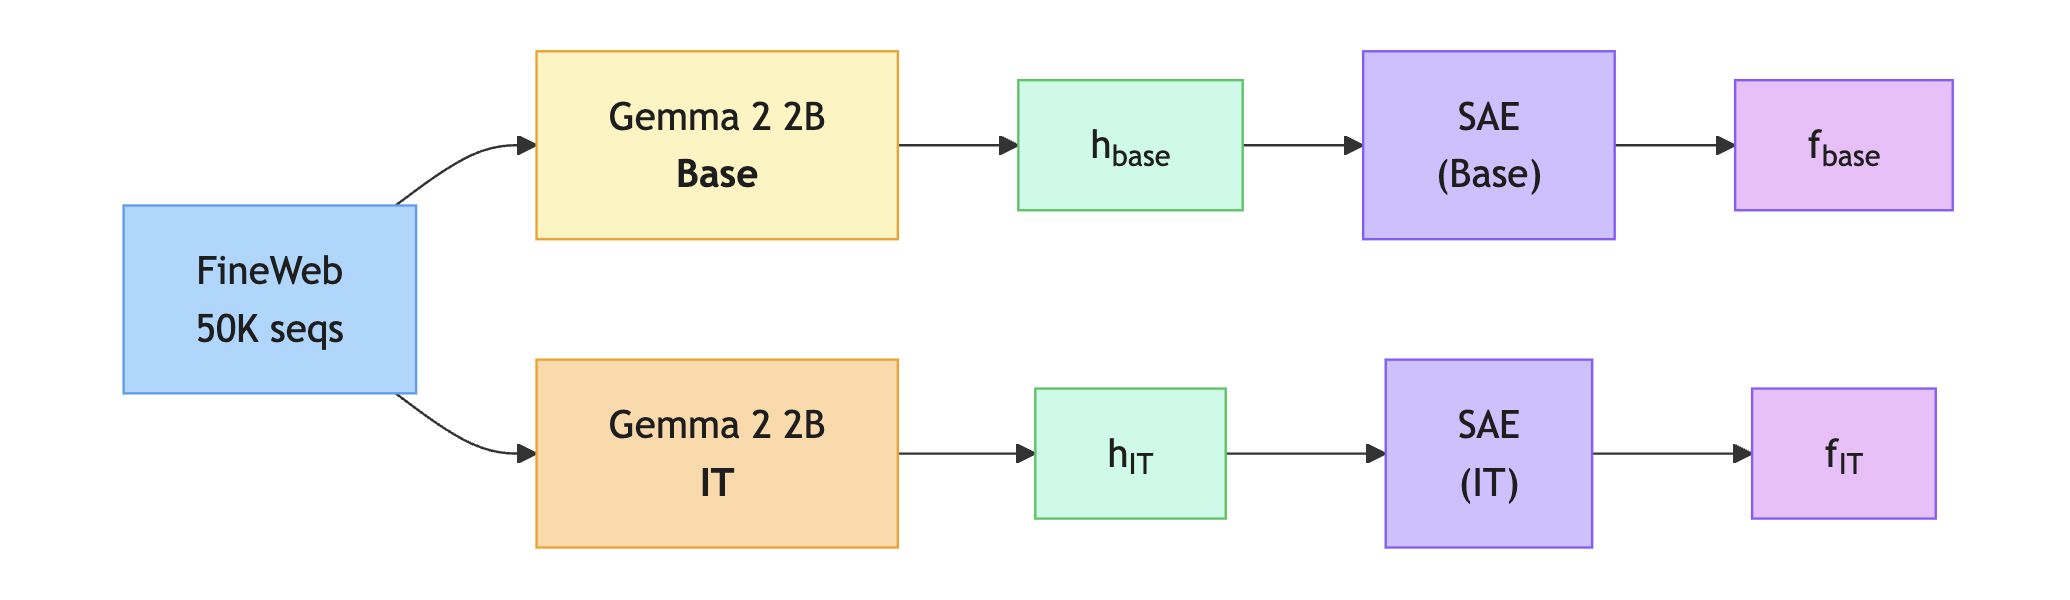
\includegraphics[width=\textwidth]{Diagram 1 - Data & Activation Collection.png}
    \caption{Data and activation collection pipeline. Identical FineWeb sequences are processed by both the PT and IT variants of Gemma 3 1B, and the residual stream at layer 13 is decomposed into sparse feature vectors by the corresponding Gemma Scope 2 SAEs.}
    \label{fig:data-activation-collection}
\end{figure}

\begin{figure}[htbp]
    \centering
    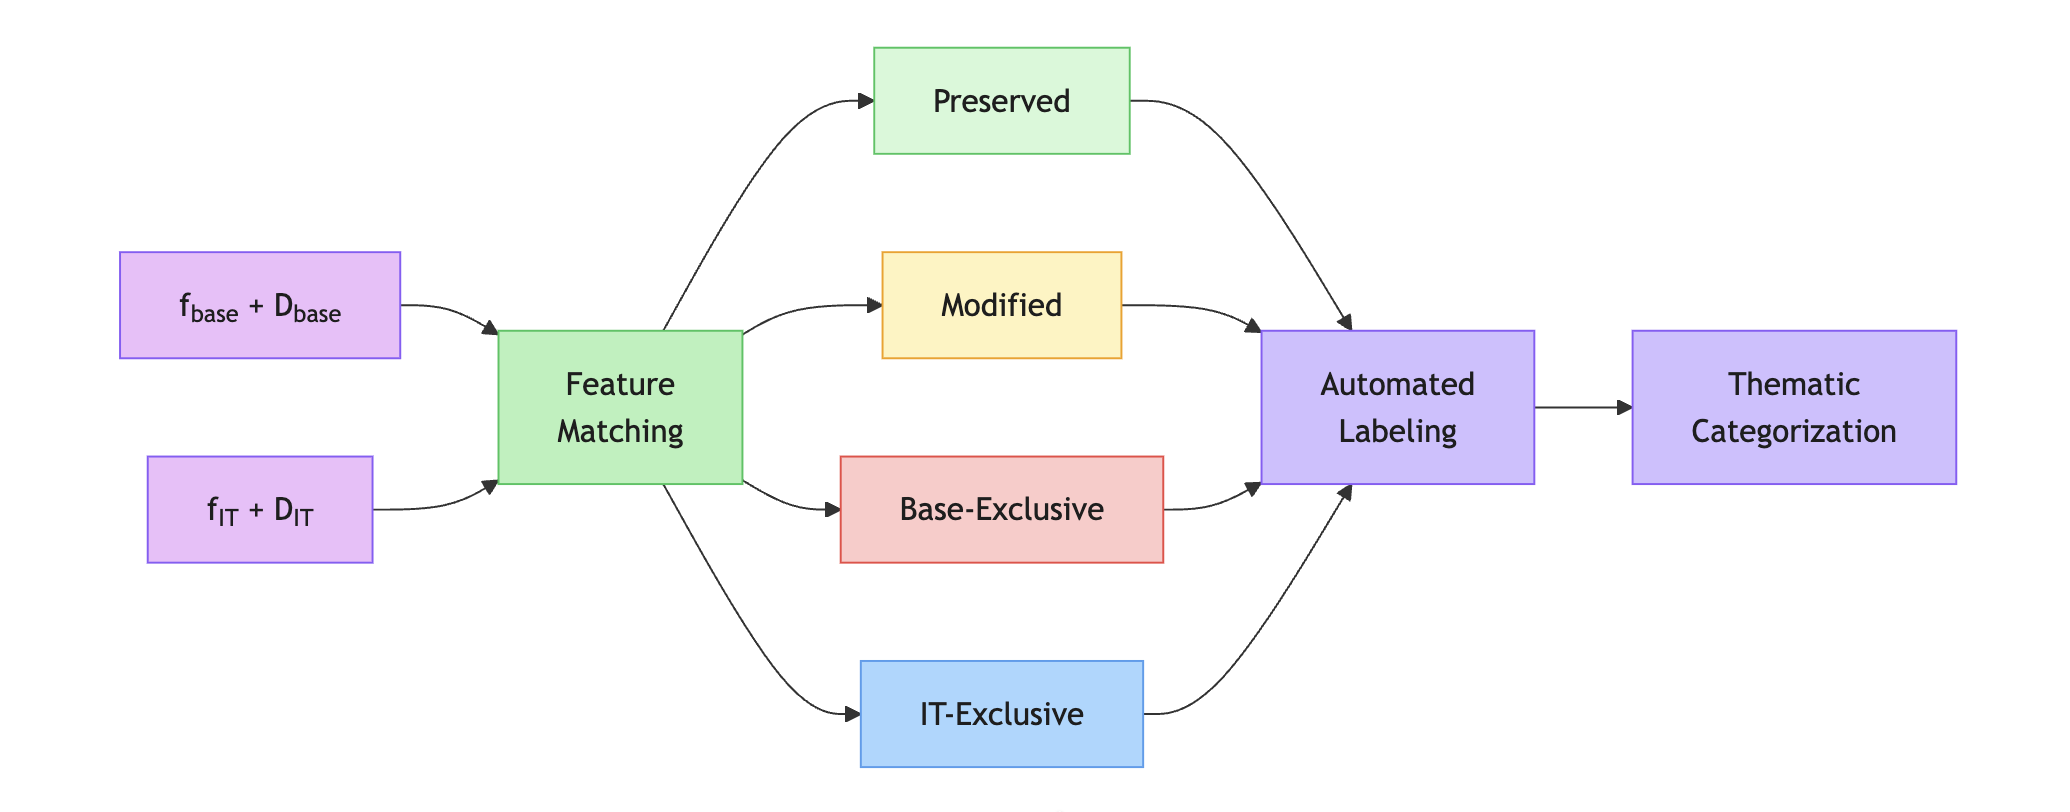
\includegraphics[width=\textwidth]{Diagram 2 - Feature Comparison.png}
    \caption{Feature comparison pipeline. Layer-13 sparse feature vectors and decoder matrices from both models are matched across PT and IT, then classified into preserved, modified, PT-exclusive, and IT-exclusive categories before targeted analysis and labelling.}
    \label{fig:feature-comparison}
\end{figure}

\begin{figure}[htbp]
    \centering
    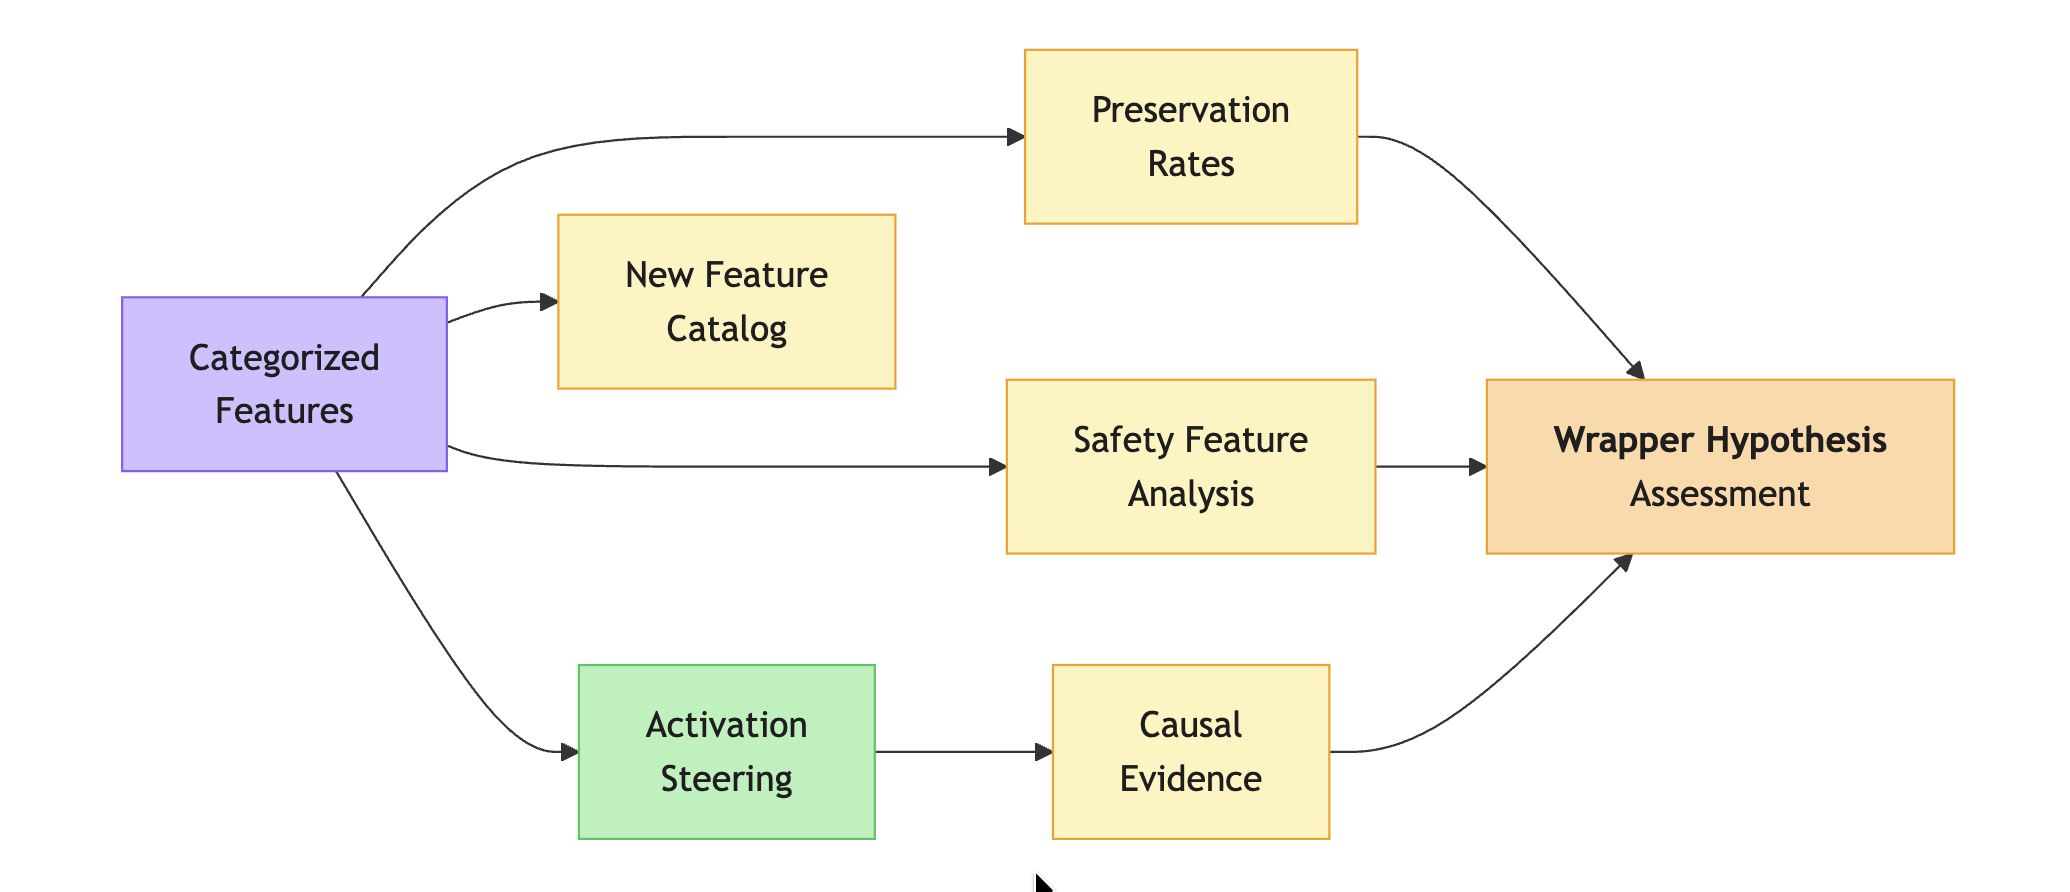
\includegraphics[width=\textwidth]{Diagram 3 - Validation & Results.png}
    \caption{Validation and results pipeline. Categorised features feed into threshold sensitivity analysis, targeted safety and instruction probing, and causal verification through activation steering, converging on an empirical test of the wrapper hypothesis.}
    \label{fig:validation-results}
\end{figure}

\subsection{Models and SAEs}
\label{subsec:models-saes}

\textbf{Models.} Gemma 3 1B is treated here as a dense decoder-only transformer with 26 layers and a hidden dimension of 1152. The base variant, \texttt{gemma-3-1b-pt}, is pre-trained only; the instruction-tuned variant, \texttt{gemma-3-1b-it}, shares the same backbone but has additionally undergone Google's standard post-training pipeline. Both models are loaded in \texttt{bfloat16}. Earlier tests with \texttt{float16} produced NaN activations at layer 13 due to overflow, which the larger dynamic range of \texttt{bfloat16} avoids.

\textbf{SAEs.} Both PT and IT models use the corresponding Gemma Scope 2 residual-stream SAEs at layer 13, with release strings \texttt{gemma-scope-2-1b-pt-res} and \texttt{gemma-scope-2-1b-it-res}, and SAE id \texttt{layer\_13\_width\_16k\_l0\_medium}. These are JumpReLU SAEs with a dictionary width of 16,384 features, approximately 14 times the model hidden dimension, trained independently on activations from each model variant \parencite{rajamanoharan_improving_2024, lieberum_gemma_2024}. That independence is necessary for comparison, but it also means that the same underlying concept can be decomposed into different dictionary elements in the two models, which is precisely why the matching procedure uses two complementary criteria.

On the FineWeb sample used here, the PT SAE has mean FVU 0.066, mean $L_0 \approx 61.4$, and 8,142 features active on more than 0.1\% of tokens. The IT SAE has mean FVU 0.124, mean $L_0 \approx 65.1$, and 4,828 features active on more than 0.1\% of tokens. The higher FVU and smaller pool of live features in the IT SAE is itself interpreted as a substantive result: post-training appears to narrow the effective feature inventory at this layer, concentrating activation mass on fewer dictionary elements.

\subsection{Data and Activation Collection}
\label{subsec:data-activation}

\textbf{Corpus.} A random sample of 5,000 sequences from FineWeb is drawn, each truncated to 256 tokens. Sequences shorter than 256 tokens are discarded rather than padded. This yields 1,275,000 valid activation positions once the first BOS token is dropped from each sequence. The sample size is reduced from the 50,000 sequences proposed in the original draft because the dual-LLM labelling and steering stages added compute requirements that were not part of the original scope, and threshold sensitivity analysis showed that the qualitative results stabilise well within a 5K-sequence sample.

\textbf{Tokenisation.} The Gemma 3 tokenizer is shared across PT and IT, so identical text produces identical token sequences in both models. Prompts are passed as raw text without applying the IT chat template, since doing so would introduce special tokens the base model has never seen and would confound the comparison.

\textbf{Activation extraction.} A forward hook on \texttt{model.model.layers[13]} captures the residual-stream output for every position in every sequence. Because the SAE is trained on float32 activations, hidden states are cast back from \texttt{bfloat16} to float32 before encoding. To stay within the VRAM budget, activations are moved to CPU after extraction and then streamed back to GPU in chunks of 64 tokens for SAE encoding, while running sums are accumulated incrementally rather than storing the full activation tensor.

\subsection{Feature Matching and Classification}
\label{subsec:feature-matching}

\textbf{Decoder-direction similarity.} Both decoder matrices are $L_2$-normalised along the feature dimension. For each PT feature $i$, the cosine similarity to every IT decoder direction $j$ is computed in chunks of 1,024 features, and the highest-similarity IT counterpart is recorded. The same is done in the reverse direction because the matching is not assumed to be symmetric. The aggregate Mean Maximum Cosine Similarity values are 0.634 for PT$\rightarrow$IT and 0.626 for IT$\rightarrow$PT. These are moderate values and well below the level one would expect under strict feature preservation.

\textbf{Activation correlation.} For each best-match pair, the Pearson correlation between the two features' per-sequence mean activation vectors of length 5,000 is computed. Per-sequence rather than per-token activations are used because storing full per-token vectors would exceed the available memory budget and because downstream labelling and targeted analysis also operate on per-sequence means. Mean activation correlation is 0.150, with median 0.006, indicating that the bulk of features show low cross-model agreement on firing pattern even when their geometric directions are similar.

\textbf{Classification.} A feature is classified as \textit{preserved} when both criteria exceed their thresholds, \textit{modified} when exactly one does, \textit{PT-exclusive} when neither holds from the PT side, and \textit{IT-exclusive} when neither holds from the IT side. Only features active on at least 0.1\% of tokens enter the counts, so dead features are excluded. The primary thresholds adopted for downstream analysis are $\tau_d = 0.7$ and $\tau_a = 0.3$, yielding 241 preserved features (3.0\% of active PT), 4,017 modified (49.3\%), 3,884 PT-exclusive (47.7\%), and 1,899 IT-exclusive (39.3\% of active IT). Under the stricter literature-style thresholds $\tau_d = 0.8$ and $\tau_a = 0.7$, the preserved category collapses to only 34 features, which makes threshold choice a central methodological issue rather than a minor implementation detail.

\subsection{Threshold Sensitivity Analysis}
\label{subsec:threshold-sensitivity}

To check whether the qualitative picture is robust, the four-way classification is recomputed on a $5 \times 5$ grid of threshold values:
\[
    \tau_d \in \{0.5, 0.6, 0.7, 0.8, 0.9\}, \qquad
    \tau_a \in \{0.1, 0.2, 0.3, 0.5, 0.7\}.
\]
Across this entire grid, the modified category exceeds 30\% of active PT features in every setting and the preserved category remains small throughout. The wrapper-hypothesis-friendly reading---that most features have a recognisable counterpart but fire differently---is therefore not a threshold artefact.

\subsection{Targeted Analysis on Safety and Instruction Prompts}
\label{subsec:targeted-analysis}

To probe behaviourally relevant features, three labelled prompt sets are loaded:
\begin{itemize}
    \item JailbreakBench JBB-Behaviors, using 100 harmful and 100 benign prompts, for safety;
    \item Stanford Alpaca, using 200 instructions, for instruction-following;
    \item the TruthfulQA generation split, using 200 questions, as a complementary factual probe.
\end{itemize}

Each prompt is tokenised, passed through both PT and IT, and its mean per-feature activation at layer 13, averaged over non-BOS tokens, is recorded. For each group-versus-baseline comparison, Welch's $t$-test identifies the features with the largest standardised mean difference between the two groups, separately in PT and IT. The top 20 features per group per model are then cross-referenced against the matching results and bucketed into ``IT-exclusive,'' ``Has PT match,'' or ``No clear match,'' giving a direct test of RQ2.

These results are persisted to \texttt{targeted\_analysis\_results.json} so that the steering stage can reuse the empirical mean activations for norm calibration.

A methodological note is important here. The original draft proposed contrasting overtly benign and overtly harmful prompts. Pilot runs showed that this gives weak diagnostic signal, because the IT model's most differentially active features often fire on lexical cues such as ``how to,'' ``create,'' or ``make'' rather than on semantic harm. Near-boundary, ambiguously framed prompts would likely provide a stronger test, and this is treated as a limitation rather than ignored.

\subsection{Automated Feature Labelling}
\label{subsec:feature-labelling}

For each feature category---preserved, modified, PT-exclusive, and IT-exclusive---50 features are sampled and labelled. For each selected feature, the 20 highest-activating sequences from the 5K-sequence FineWeb sample are collected, with activating tokens flagged using \texttt{>>>...<<<} markers. These examples are then sent in parallel to two LLMs.

Claude Haiku 4.5 is queried through a structured-output schema that requests a free-text description, a categorical label from the set \{\texttt{language\_syntax}, \texttt{knowledge\_semantics}, \texttt{instruction\_style}, \texttt{safety\_alignment}, \texttt{formatting}, \texttt{other}\}, and a confidence rating from 1 to 5. GPT-4.1-nano is queried with the same schema and prompt. Outputs are saved separately to \texttt{feature\_labels\_claude.json} and \texttt{feature\_labels\_openai.json}.

Inter-model agreement is computed per category and yields an overall rate of about 59.5\%. Agreement is highest for preserved features and degrades as features become more ambiguous, which is the expected pattern. The two annotators most often disagree on the boundary between \texttt{language\_syntax} and \texttt{instruction\_style}, suggesting that many instruction-following cues are realised through syntactic markers. A high-confidence consensus subset is then constructed by retaining only features for which both models report confidence at least 4. This consensus list is the subset used for downstream steering selection.

Claude Haiku is preferred over a larger Anthropic model because the labelling task is essentially short-context pattern recognition, and pilot validation did not reveal a quality difference large enough to justify the cost increase.

\subsection{Causal Verification via Activation Steering}
\label{subsec:causal-verification}

Three steering cases test the causal role of selected features:
\begin{itemize}
    \item \textbf{Case A: IT-exclusive features steered in the base model.} If post-training installs genuinely new safety- or instruction-relevant features, then injecting an IT-exclusive feature into the PT model should shift outputs in the direction predicted by its label. The selected candidates are features 241, 222, 2006, and 446.
    \item \textbf{Case B: PT-exclusive features steered in the IT model.} If post-training suppresses pre-existing capabilities rather than removing them, then re-injecting a PT-exclusive feature into the IT model should re-surface the corresponding behaviour. The selected candidates are features 329 and 75.
    \item \textbf{Case C: dose-response on modified features.} Two features classified as modified, 222 and 446, are steered across a finer multiplier grid in the IT model to characterise the relationship between intervention magnitude and behavioural change.
\end{itemize}

\textbf{Steering implementation.} A forward hook on layer 13 adds $\alpha \cdot \mathbf{d}_i$ to the residual stream during generation, where $\mathbf{d}_i$ is the SAE decoder column for feature $i$. Decoder directions are taken at their learned SAE scale rather than unit-normalised, because unit normalisation would discard empirically learned magnitude information and make $\alpha$ less interpretable across features.

\textbf{Norm calibration of $\alpha$.} Pilot runs at a fixed $\alpha = 50$ produced almost no behavioural change because the residual-stream norms at layer 13 of Gemma 3 1B are large. Instead, $\alpha$ is parameterised relative to the empirical mean activation of the target feature, taken from the targeted analysis:
\[
    \alpha = m \times \text{mean\_act},
\]
with multipliers $m \in \{-5, -3, -1, 0, 1, 3, 5, 10\}$ for Cases A and B, and $m \in \{-10, -5, -3, -1, 0, 1, 3, 5, 10, 20\}$ for Case C. This makes the intervention interpretable as a multiple of the feature's natural firing strength.

\textbf{Evaluation.} Two evaluation metrics are used:
\begin{enumerate}
    \item KL divergence between the next-token distributions of steered and unsteered generations at the final prompt position;
    \item qualitative text-change classification, where steered and unsteered 60-token generations are compared as strings and tagged either \texttt{CHANGED} or \texttt{same}.
\end{enumerate}
Each feature is tested across nine prompts spanning instruction, safety, and neutral settings for Cases A and B, and across three prompts for Case C.

\subsection{Implementation Notes}
\label{subsec:implementation-notes}

All experiments are conducted in Python in a Jupyter notebook on a single GPU with roughly 79 GB VRAM. Models are loaded in \texttt{bfloat16}; SAE encoding runs in float32 to match Gemma Scope training precision. The random seed is fixed at 42 for sampling and prompt ordering. SAELens is used for SAE loading and steering hooks, the Anthropic Python SDK for structured Claude outputs, and OpenAI's official client for GPT-4.1-nano labelling. Intermediate artefacts---classification masks, labels from both annotators, the consensus list, the targeted analysis JSON, and the steering results JSON---are all written to disk so that later stages can be rerun independently.

\subsection{Assumptions, Limitations, and Scope}
\label{subsec:assumptions-limitations}

The methodology rests on the linear representation hypothesis and on the adequacy of Gemma Scope 2 SAEs as a feature extractor. Both are tested only indirectly: the former through the coherence of automated labels and the latter through reported FVU values. The main limitations are as follows.

\begin{itemize}
    \item \textbf{Single layer, single model pair, single scale.} Findings are valid for layer 13 of Gemma 3 1B with the 16K-width Gemma Scope 2 SAEs and need not generalise to other layers, larger Gemma variants, or other architectures.
    \item \textbf{Reduced sample size.} The study uses 5K FineWeb sequences rather than the 50K proposed in the original draft. Threshold sensitivity is robust within this sample, but rare-feature statistics are necessarily weaker.
    \item \textbf{Per-sequence rather than per-token correlation.} Activation correlation is computed on per-sequence mean activations to fit in memory, which can under-count features that match locally but not globally.
    \item \textbf{Raw decoder norms in steering.} Steering uses raw, not unit-normalised, decoder directions. This preserves learned SAE scale but requires the multiplier-by-mean-activation calibration to keep interventions interpretable.
    \item \textbf{KL at a single position.} Variable generation lengths under steering make a full-generation KL window ill-defined, so KL is reported only at the final prompt token.
    \item \textbf{Prompt selection.} The targeted prompts are categorical contrasts rather than near-boundary probes. A stronger safety diagnosis would likely come from more ambiguous prompts.
    \item \textbf{Crosscoders are out of scope.} A PT-vs-IT crosscoder for Gemma 3 would eliminate post-hoc matching entirely, but currently published Gemma Scope crosscoders are cross-layer rather than cross-model, so that extension is left for future work.
\end{itemize}

\section{Technical Content and Key Results}
\label{sec:results}

\subsection{Macroscopic Picture (RQ1)}
\label{subsec:rq1-results}

At the strict literature thresholds $\tau_d = 0.8$ and $\tau_a = 0.7$, only 34 of the 8,142 active PT features at layer 13 are preserved, approximately 0.4\%. A further 2,436 features, or 29.9\%, are modified; 5,672, or 69.7\%, are PT-exclusive; and 3,407 of the 4,828 active IT features, or 70.6\%, are IT-exclusive. Mean MMCS is 0.634 for PT$\rightarrow$IT, well below the level one would expect under strict feature reuse.

At the moderate thresholds used as the primary setting, $\tau_d = 0.7$ and $\tau_a = 0.3$, the shape changes but the message does not: 241 features are preserved (3.0\%), 4,017 are modified (49.3\%), 3,884 are PT-exclusive (47.7\%), and 1,899 are IT-exclusive (39.3\%). The modified category is now the largest single bucket, which is exactly the wrapper-hypothesis prediction: most features have a recognisable cross-model counterpart, but their firing patterns differ.

The threshold sensitivity sweep strengthens that reading. The modified category exceeds 30\% of active PT features across the entire $5 \times 5$ grid, while the preserved category never rises above 12\%. The qualitative dominance of modified over preserved is therefore not a threshold artefact.

\subsection{Labelling and Cross-Model Consensus}
\label{subsec:labelling-results}

Fifty features per category are labelled by both Claude Haiku 4.5 and GPT-4.1-nano. Inter-model agreement on the categorical label is 74\% for preserved features, 54\% for modified, 44\% for PT-exclusive, and 48\% for IT-exclusive. This is a clean monotonic pattern: the more ambiguous the matching status, the harder the semantic labelling task.

Claude's labels for IT-exclusive features lean strongly toward \texttt{language\_syntax} and \texttt{formatting}, with very few in \texttt{instruction\_style} and none in \texttt{safety\_alignment}. GPT-4.1-nano yields a flatter distribution over the same sample. Neither model spontaneously identifies a meaningful number of IT-exclusive safety features in the labelling sample. That is itself a non-trivial result, because a strong creation-based interpretation of post-training would predict the opposite.

The high-confidence consensus list, defined by confidence at least 4 from both models, contains 14 IT-exclusive features, 13 PT-exclusive, 22 modified, and 37 preserved. This consensus subset is what feeds the targeted analysis and steering stages.

\subsection{Targeted Differential Analysis (RQ2)}
\label{subsec:rq2-results}

Welch's $t$-test on JailbreakBench harmful-versus-benign prompts surfaces 20 features per model. When the IT-side top-20 safety features are looked up in the matching results, 5 have a clear PT match, 3 are IT-exclusive, and 12 fall into a no-clear-match zone where only one matching criterion is satisfied. Repeating the same exercise on Alpaca instruction prompts yields 7 with a PT match, 6 IT-exclusive, and 7 ambiguous.

This is the central empirical result of the thesis. If post-training had installed new safety- and instruction-relevant features as discrete entities, the top differential IT features should overwhelmingly have been IT-exclusive. They are not. The largest bucket is the ambiguous or modified zone, and clear PT matches outnumber clear IT-exclusives in both probes. On this evidence, post-training is re-weighting features the base model already had, which is precisely the wrapper prediction.

\subsection{Causal Verification via Steering (RQ3)}
\label{subsec:rq3-results}

\textbf{Case A: IT-exclusive features steered in PT.} Feature 241, with mean activation 173.3 and labelled as a wrongdoing or harmful-activity detector, produces graded behavioural changes when injected into the base model. At multiplier $m = +3$, corresponding to $\alpha \approx +520$, KL divergence ranges from 0.03 to 0.06 and 5 of 9 generations differ visibly from baseline. At $m = +10$, with $\alpha \approx +1733$, KL reaches 0.4 to 0.96 and all 9 generations differ. Importantly, the qualitative effect is not ``the base model started refusing harmful prompts'' but rather ``the base model became more verbose, more first-person, and more prone to topic drift.'' Features 222, 446, and 2006 show smaller but qualitatively similar effects. The feature is therefore causal, but its label appears to describe a firing condition rather than a full behavioural target.

\textbf{Case B: PT-exclusive features steered in IT.} Features 329 and 75 produce monotonic dose-response curves under both positive and negative steering, with KL values from approximately 0 at $m = \pm 1$ to about 0.03 at $m = \pm 10$. Steering is therefore causal on output distributions even for features that the matching pipeline labelled as PT-exclusive, which suggests that the IT model remains sensitive to these directions even though its own SAE dictionary did not learn dedicated counterparts for them.

\textbf{Case C: modified features in IT.} Features 222 and 446 produce clean monotonic dose-response curves inside the IT model itself: KL is around $10^{-3}$ at $m = \pm 1$, around $10^{-2}$ at $m = \pm 5$, and between 0.46 and 0.84 at $m = +20$. All three generations differ at $m = +10$ and $m = +20$ for both features. This is the clearest evidence for the modulation reading: the feature direction is shared across PT and IT, but its natural firing strength is what post-training tunes.

Taken together, the steering results support a graded version of the wrapper hypothesis. Post-training does not appear to create discrete new safety circuits at layer 13 of Gemma 3 1B. Instead, it adjusts the firing patterns and effective strengths of features that already exist as directions in the base model's residual stream.

\section{Limitations and Robustness}
\label{sec:limitations-robustness}

The threshold sensitivity sweep covers the main free parameter in the matching procedure and shows that the qualitative result, modified greater than preserved throughout, is robust. The dual-LLM labelling protocol guards against single-annotator bias, and the consensus filter discards ambiguous cases. Norm-calibrated steering uses empirical mean activations rather than fixed $\alpha$ values, controlling for large cross-feature variation in natural firing magnitudes.

The main remaining sources of uncertainty are exactly those already declared in the methodology: single layer, single model pair, reduced sample size, per-sequence rather than per-token correlation, raw decoder norms in steering, single-position KL, and overtly categorical targeted prompts. None of these would be expected to reverse the central conclusion on present evidence. The modified category is too dominant, and the targeted analysis too one-sided, for a small methodological tweak to flip the result. But each limitation constrains how broadly the conclusion can be claimed to hold.

The most consequential limitation is the single-layer scope. \textcite{du_how_2025} report that post-training effects vary substantially across depth, and a more complete picture would therefore require the same analysis to be repeated at an early layer, a mid layer, and a late layer. That is the clearest next step.

\section{Conclusions, Implications, and Application to the Real World}
\label{sec:conclusions}

The empirical answer this thesis arrives at is straightforward: at layer 13 of Gemma 3 1B, instruction tuning predominantly reorganises features the base model already had rather than installing new ones. Three independent lines of evidence converge on that conclusion. First, the matching results show that under every threshold setting in the $5 \times 5$ grid the modified category vastly outnumbers the preserved category, meaning that most features have a cross-model counterpart but a different firing pattern. Second, when IT-side features are surfaced by safety and instruction probes, the largest bucket is ``matched to a PT feature'' rather than ``IT-exclusive.'' Third, steering both IT-exclusive and modified features produces graded behavioural change, but that change reads as modulation rather than the introduction of a new behavioural primitive.

\textbf{Implications for alignment research.} If this picture generalises, then interventions that aim to ``remove safety features'' or ``find the refusal feature'' are looking for the wrong kind of object. The relevant unit is not a discrete post-training-introduced feature but a modulation pattern over pre-existing features. That reframes a substantial portion of the alignment-by-interpretation programme: red-teaming should assume capabilities are never deleted, only down-weighted; defences should target activation distributions rather than feature presence; and crosscoder-style joint dictionaries are likely to be the right tool for the job because they make modulation explicit by construction.

\textbf{Practical takeaway for practitioners.} The pipeline released alongside this thesis can be rerun on future paired base/IT releases whenever Gemma-Scope-style SAEs become available. The dual-LLM consensus protocol generalises naturally to other feature-labelling tasks and is inexpensive enough for student-budget experimentation. The norm-calibrated steering convention, $\alpha = m \times \text{mean\_activation}$, yields interventions that are more interpretable than fixed raw-vector magnitudes and may therefore be useful beyond this particular thesis.

\textbf{Future work.} Three extensions are immediate: repeat the analysis at early and late layers to recover the depth profile; train a PT-vs-IT crosscoder for Gemma 3 1B to validate the matching results against a method that does not need post-hoc matching; and rerun the targeted analysis on near-boundary safety prompts to test whether the apparent absence of dedicated safety features survives a stronger probe.

On the evidence presented here, the wrapper hypothesis is not merely a convenient metaphor. It is a testable empirical claim about how post-training reshapes language models, and at layer 13 of Gemma 3 1B it survives the test.


\clearpage
\appendix
\section{Literature Review Summary}
\label{sec:appendix-literature-summary}

This appendix summarises the studies that most directly motivate the research design and clarifies how each contributes to the present project.

\begin{itemize}
    \item \textbf{Elhage et al.\ (2022)} \parencite{elhage_toy_2022} establish the superposition framework, explaining why individual neurons are often polysemantic and why neuron-level interpretability is limited.
    \item \textbf{Templeton et al.\ (2024)} \parencite{templeton_scaling_2024} demonstrate that sparse autoencoders can recover large numbers of interpretable, causally meaningful features from frontier language models, making feature-level comparison feasible.
    \item \textbf{Ouyang et al.\ (2022)} \parencite{ouyang_training_2022} show that post-training techniques such as supervised fine-tuning and RLHF can strongly improve instruction-following, helpfulness, and safety.
    \item \textbf{Zhou et al.\ (2023)} \parencite{zhou_lima_2023} argue that most capability is learned during pre-training and that a relatively small amount of fine-tuning data can substantially reshape model behaviour, motivating the superficial alignment hypothesis.
    \item \textbf{Du et al.\ (2025)} \parencite{du_how_2025} provide direct mechanistic evidence that post-training affects some behavioural directions, especially refusal, more than core factual knowledge representations.
\end{itemize}

\section{Implications for the Present Study}
\label{sec:appendix-literature-implications}

The literature review motivates the methodology in three ways.

\begin{itemize}
    \item It justifies the use of sparse autoencoders as the main interpretability tool, because superposition makes individual neurons an unreliable unit of analysis.
    \item It motivates comparing a base model with its instruction-tuned counterpart, because post-training is the stage where alignment-relevant behavioural changes are introduced.
    \item It frames the core empirical question of the project: whether post-training creates new interpretable features, suppresses existing ones, or primarily changes the activation patterns of a largely preserved feature set.
\end{itemize}


\clearpage
\printbibliography

\end{document}
